\documentclass[11pt,fleqn]{article}
\usepackage{../cs188,latexsym,epsf, amsmath,amsfonts,graphicx,url,multicol}
\lecture{2}
\def\title{Note \the\lecturenumber}
\begin{document}
\maketitle


\iffalse
\documentclass[11pt,fleqn]{article}
\usepackage{latexsym,epsf,amsmath,amsfonts,graphicx,url}

\title{Note 2}

\newcommand{\F}{\mathbb{F}}
\newcommand{\Z}{\mathbb{Z}}
\newcommand{\Q}{\mathbb{Q}}
\newcommand{\R}{\mathbb{R}}
\newcommand{\C}{\mathbb{C}}

\begin{document}

\maketitle
\fi

\section*{Constraint Satisfaction Problems}
In the previous note, we learned how to find optimal solutions to search problems, a type of \textbf{planning problem}. Now, we'll learn about solving a related class of problems, \textbf{constraint satisfaction problems} (CSPs). Unlike search problems, CSPs are a type of \textbf{identification problem}, problems in which we must simply identify whether a state is a goal state or not, with no regard to how we arrive at that goal. CSPs are defined by three factors:
	\begin{enumerate}
		\item \textit{Variables} - CSPs possess a set of $N$ variables $X_1, ..., X_N$ that can each take on a single value from some defined set of values.
		\item \textit{Domain} - A set $\{x_1, ..., x_d\}$ representing all possible values that a CSP variable can take on.
		\item \textit{Constraints} - Constraints define restrictions on the values of variables, potentially with regard to other variables.
	\end{enumerate}
Consider the $N$-queens identification problem: given an $N \times N$ chessboard, can we find a configuration in which to place $N$ queens on the board such that no two queens attack each another?
\begin{center}
	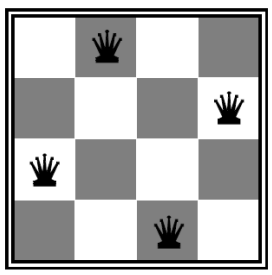
\includegraphics[width=3.7cm]{img/n-queens}
\end{center}
We can formulate this problem as a CSP as follows:
	\begin{enumerate}
		\item \textit{Variables} - $X_{ij}$, with $0 \leq i, j < N$. Each $X_{ij}$ represents a grid position on our $N \times N$ chessboard, with $i$ and $j$ specifying the row and column number respectively.
		\item \textit{Domain} - $\{0, 1\}$. Each $X_{ij}$ can take on either the value $0$ or $1$, a boolean value representing the existence of a queen at position $(i, j)$ on the board.
		\item \textit{Constraints} - 
			\begin{itemize}
				\item $\forall i,j,k \:\: (X_{ij}, X_{ik}) \in \{(0, 0), (0, 1), (1, 0)\}$. This constraint states that if two variables have the same value for $i$, only one of them can take on a value of 1. This effectively encapsulates the condition that no two queens can be in the same row.
				\item $\forall i,j,k \:\: (X_{ij}, X_{kj}) \in \{(0, 0), (0, 1), (1, 0)\}$. Almost identically to the previous constraint, this constraint states that if two variables have the same value for $j$, only one of them can take on a value of 1, encapsulating the condition that no two queens can be in the same column.
				\item $\forall i,j,k \:\: (X_{ij}, X_{i+k,j+k}) \in \{(0, 0), (0, 1), (1, 0)\}$. With similar reasoning as above, we can see that this constraint and the next represent the conditions that no two queens can be in the same major or minor diagonals, respectively.
				\item $\forall i,j,k \:\: (X_{ij}, X_{i+k,j-k}) \in \{(0, 0), (0, 1), (1, 0)\}$.
				\item $\sum\limits_{i,j}X_{ij} = N$. This constraint states that we must have exactly $N$ grid positions marked with a $1$, and all others marked with a $0$, capturing the requirement that there are exactly $N$ queens on the board.
			\end{itemize}
	\end{enumerate}
Constraint satisfaction problems are \textbf{NP-complete}, which loosely means that there exists no known algorithm for finding solutions to them in polynomial time. Given a problem with $N$ variables with domain of size $O(d)$ for each variable, there are $O(d^N)$ possible assignments, exponential in the number of variables. We can often get around this caveat by formulating CSPs as search problems, defining states as \textbf{partial assignments} (variable assignments to CSPs where some variables have been assigned values while others have not). Correspondingly, the successor function for a CSP state outputs all states with one new variable assigned, and the goal test verifies all variables are assigned and all constraints are satisfied in the state it's testing. Constraint satisfaction problems tend to have significantly more structure than traditional search problems, and we can exploit this structure by combining the above formulation with appropriate heuristics to hone in on solutions in a feasible amount of time.

\subsection*{Constraint Graphs}
Let's introduce a second CSP example: map coloring. Map coloring solves the problem where we're given a set of colors and must color a map such that no two adjacent states or regions have the same color.
	\begin{center}
		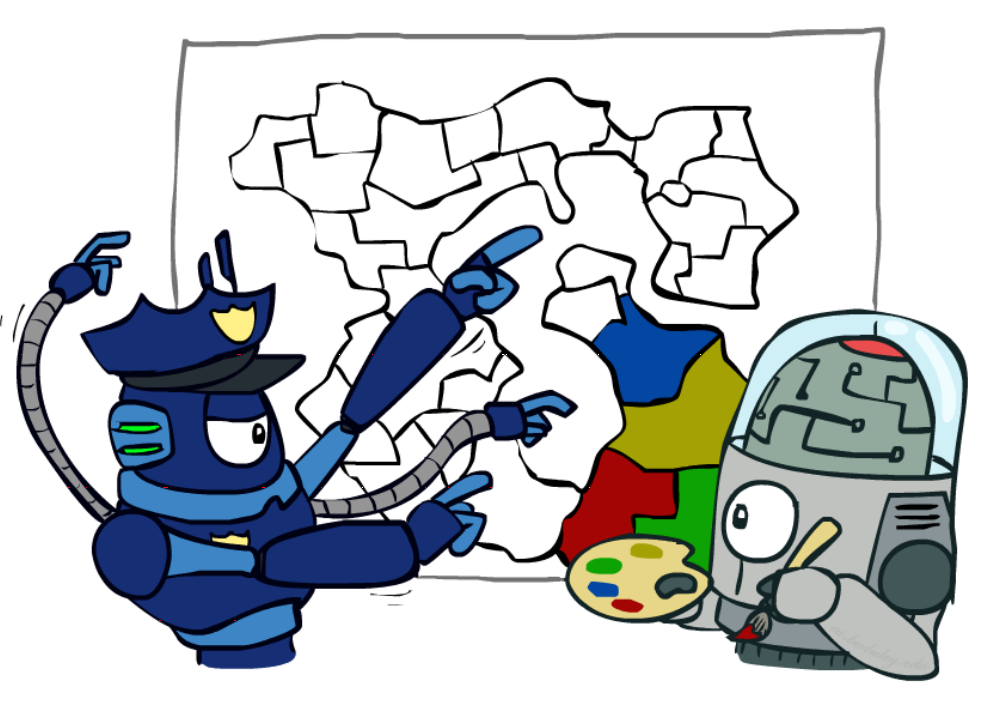
\includegraphics[width=7.5cm]{img/map-coloring-comic}
	\end{center}
Constraint satisfaction problems are often represented as constraint graphs, where nodes represent variables and edges represent constraints between them. There are many different types of constraints, and each is handled slightly differently:
\begin{itemize}
	\item \textit{Unary Constraints} - Unary constraints involve a single variable in the CSP. They are not represented in constraint graphs, instead simply being used to prune the domain of the variable they constrain when necessary.
	\item \textit{Binary Constraints} - Binary constraints involve two variables. They're represented in constraint graphs as traditional graph edges.
	\item \textit{Higher-order Constraints} - Constraints involving three or more variables can also be represented with edges in a CSP graph, they just look slightly unconventional.
\end{itemize} 
Consider map coloring the map of Australia:
	\begin{center}
		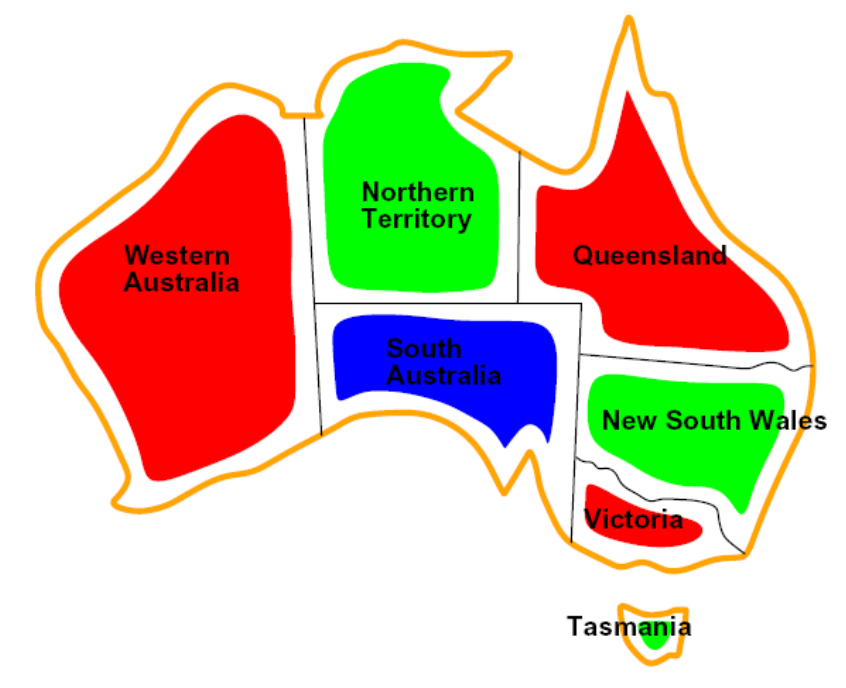
\includegraphics[width=7.5cm]{img/australia-map}
	\end{center}
The constraints in this problem are simply that no two adjacent states can be the same color. As a result, by drawing an edge between every pair of states that are adjacent to one another, we can generate the constraint graph for the map coloring of Australia as follows:
	\begin{center}
		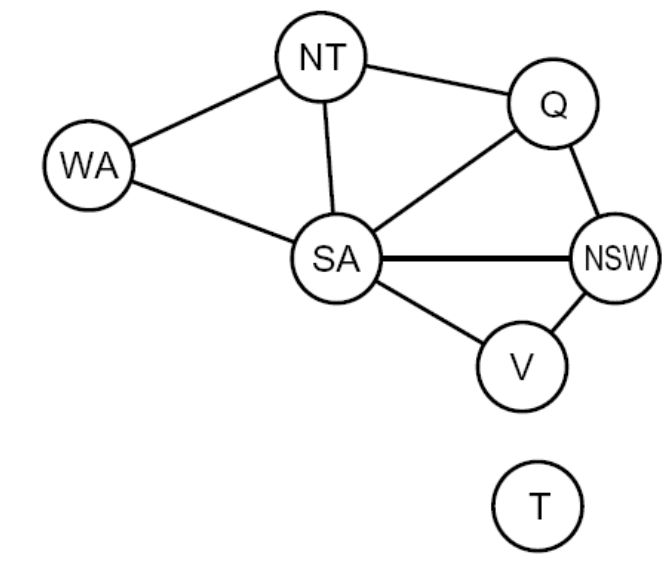
\includegraphics[width=7.5cm]{img/australia-graph}
	\end{center}
The value of constraint graphs is that we can use them to extract valuable information about the structure of the CSPs we are solving. By analyzing the graph of a CSP, we can determine things about it like whether it's sparsely or densely connected/constrained and whether or not it's tree-structured. We'll cover this more in depth as we discuss solving constraint satisfaction problems in more detail.

\section*{Solving Constraint Satisfaction Problems}
Constraint satisfaction problems are traditionally solved using a search algorithm known as \textbf{backtracking search}. Backtracking search is an optimization on depth first search used specifically for the problem of constraint satisfaction, with improvements coming from two main principles:
	\begin{enumerate}
		\item Fix an ordering for variables, and select values for variables in this order. Because assignments are commutative (e.g. assigning $WA = Red,\:\: NT = Green$ is identical to $NT = Green,\:\: WA = Red$), this is valid. 
		\item When selecting values for a variable, only select values that don't conflict with any previously assigned values. If no such values exist, backtrack and return to the previous variable, changing its value.
	\end{enumerate}
The pseudocode for how recursive backtracking works is presented below:
	\begin{center}
		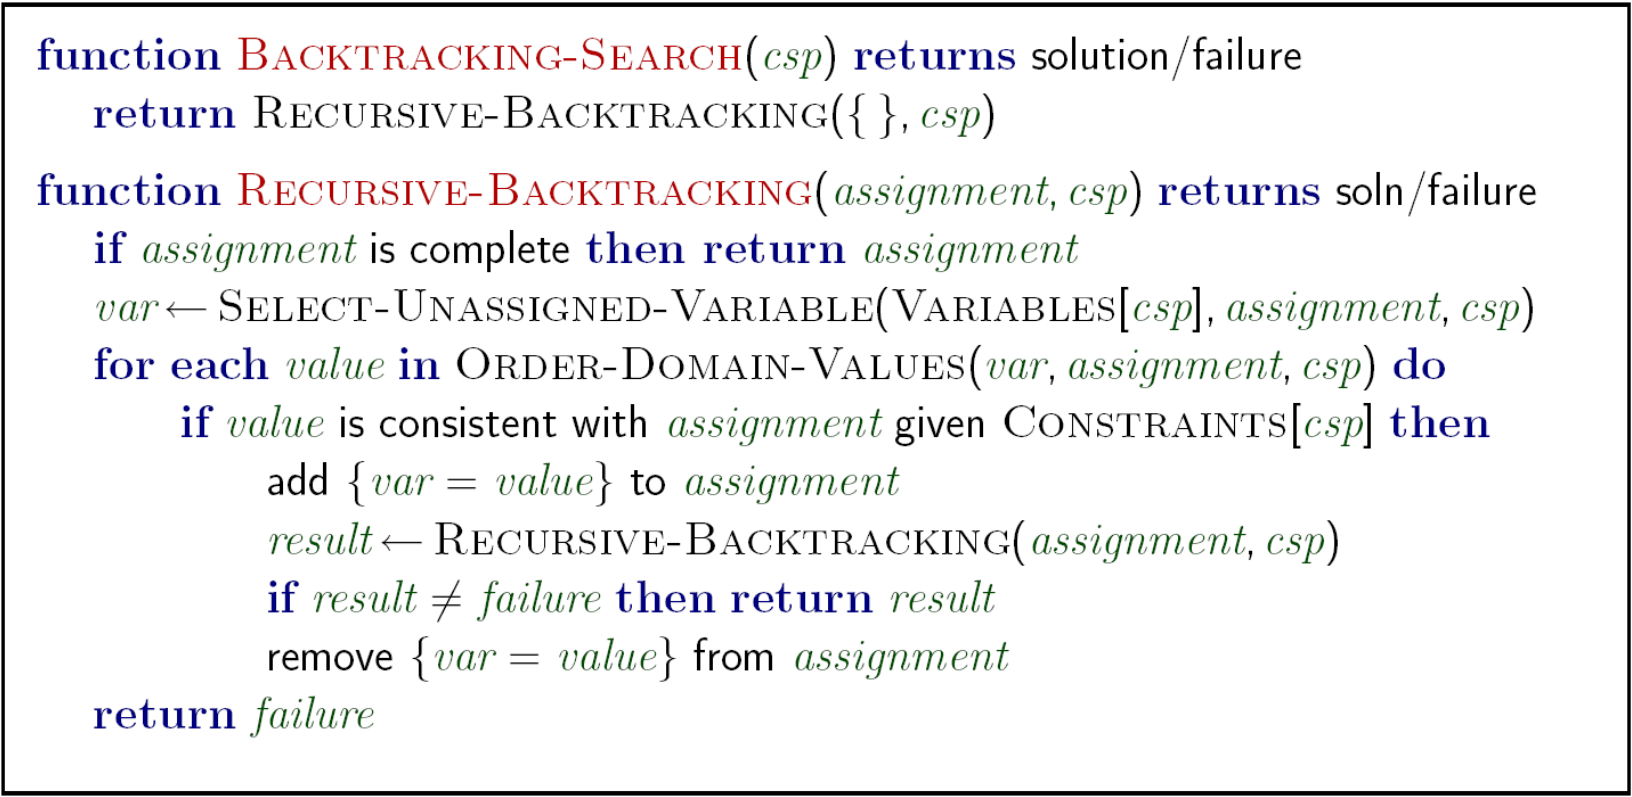
\includegraphics[width=12cm]{img/backtracking-search-pseudo.png}
	\end{center}
For a visualization of how this process works, consider the partial search trees for both depth first search and backtracking search in map coloring:
	\begin{center}
		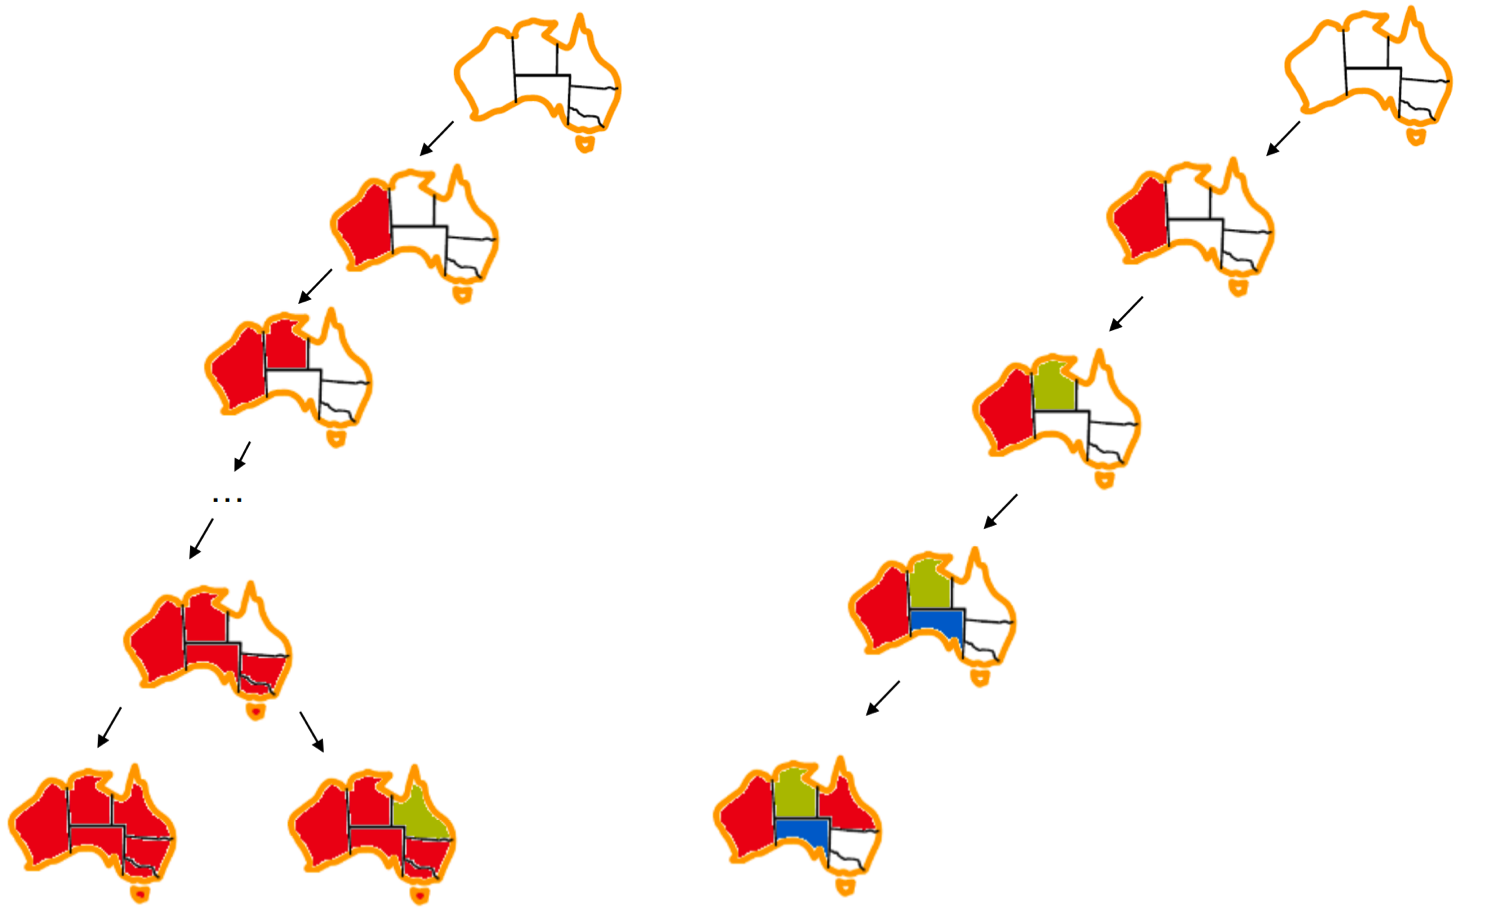
\includegraphics[width=12cm]{img/dfs-vs-backtracking.png}
	\end{center}
Note how DFS regretfully colors everything red before ever realizing the need for change, and even then doesn't move too far in the right direction towards a solution. On the other hand, backtracking search only assigns a value to a variable if that value violates no constraints, leading to a significantly less backtracking. Though backtracking search is a vast improvement over the brute-forcing of depth first search, we can get more gains in speed still with further improvements through filtering, variable/value ordering, and structural explotation. 

\subsection*{Filtering}
	The first improvement to CSP performance we'll consider is \textbf{filtering}, which checks if we can prune the domains of unassigned variables ahead of time by removing values we know will result in backtracking. A na\"{i}ve method for filtering is \textbf{forward checking}, which whenever a value is assigned to a variable $X_i$, prunes the domains of unassigned variables that share a constraint with $X_i$ that would violate the constraint if assigned. Whenever a new variable is assigned, we can run forward checking and prune the domains of unassigned variables adjacent to the newly assigned variable in the constraint graph. Consider our map coloring example, with unassigned variables and their potential values:
		\begin{center}
			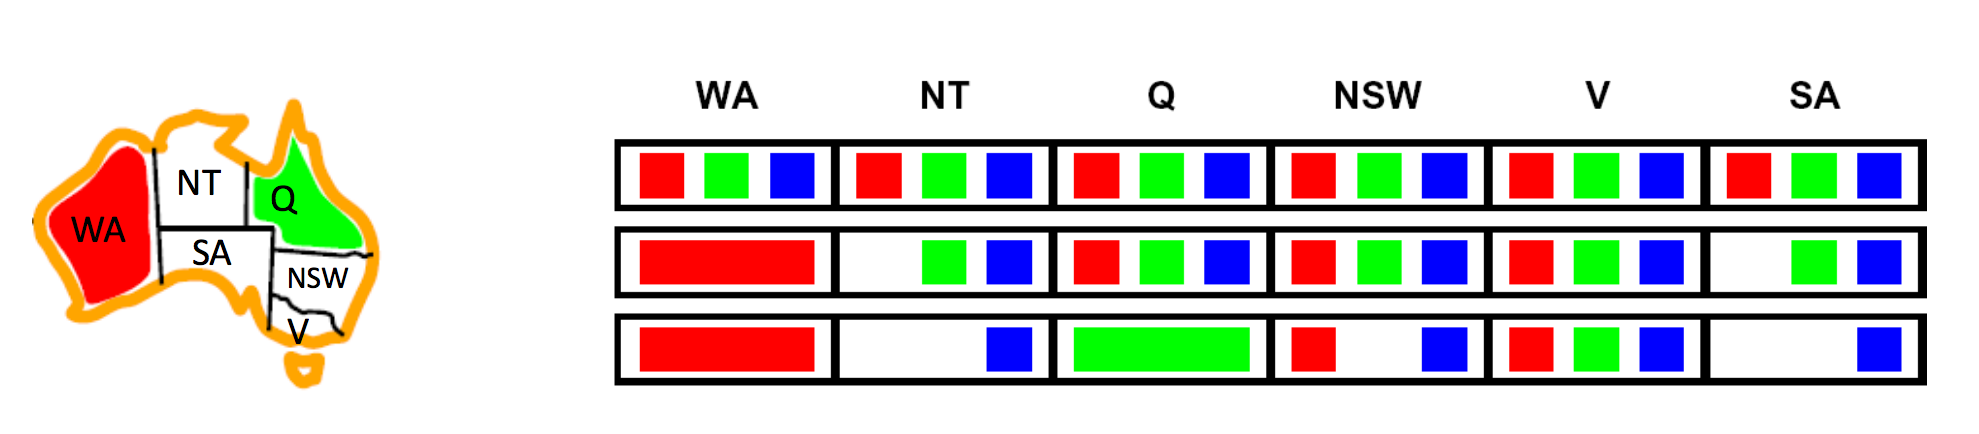
\includegraphics[width=16cm]{img/forward-checking.png}
		\end{center}
	Note how as we assign $WA = red$ and then $Q = green$, the size of the domains for $NT$, $NSW$, and $SA$ (states adjacent to $WA$, $Q$, or both) decrease in size as values are eliminated. The idea of forward checking can be generalized into the principle of \textbf{arc consistency}. For arc consistency, we interpret each undirected edge of the constraint graph for a CSP as two directed edges pointing in opposite directions. Each of these directed edges is called an \textbf{arc}. The arc consistency algorithm works as follows:
		\begin{itemize}
			\item Begin by storing all arcs in the constraint graph for the CSP in a queue $Q$.
			\item Iteratively remove arcs from $Q$ and enforce the condition that in each removed arc $X_i \longrightarrow X_j$, for every value in the domain of the tail variable $X_i$, there is at least one variable in $X_j$ that violates no constraints between $X_i$ and $X_j$.
			\item If at least one value is removed from the domain of $X_i$ when enforcing arc consistency for an arc $X_i \longrightarrow X_j$, add arcs of the form $X_k \longrightarrow X_i$ to $Q$, for all unassigned variables $X_k$. If an arc $X_k \longrightarrow X_i$ is already in $Q$ during this step, it doesn't need to be added again.
			\item Continue until $Q$ is empty, or the domain of some variable is empty and triggers a backtrack.
		\end{itemize}
		The arc consistency algorithm is typically not the most intuitive, so let's walk through a quick example with map coloring:
		\begin{center}
			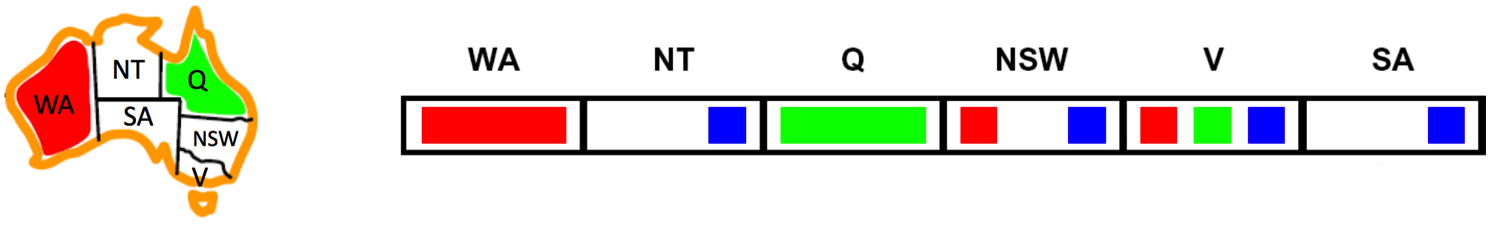
\includegraphics[width=16cm]{img/arc-consistency-ex-1.png}
		\end{center}
		We begin by adding all arcs between unassigned variables sharing a constraint to a queue $Q$, which gives us 
		\begin{eqnarray*}
		Q = [SA \rightarrow V, V \rightarrow SA, SA \rightarrow NSW, NSW \rightarrow SA, SA \rightarrow NT, NT \rightarrow SA, V \rightarrow NSW, NSW \rightarrow V]
		\end{eqnarray*}
		For our first arc, $SA \rightarrow V$, we see that for every value in the domain of $SA$, $\{blue\}$, there is \textit{at least} one value in the domain of $V$, $\{red, green, blue\}$, that violates no constraints, and so no values need to be pruned from $SA$'s domain. However, for our next arc $V \rightarrow SA$, if we set $SA = blue$ we see that $V$ will have no remaining values that violate no constraints, and so we prune $blue$ from $V$'s domain. 
		\begin{center}
			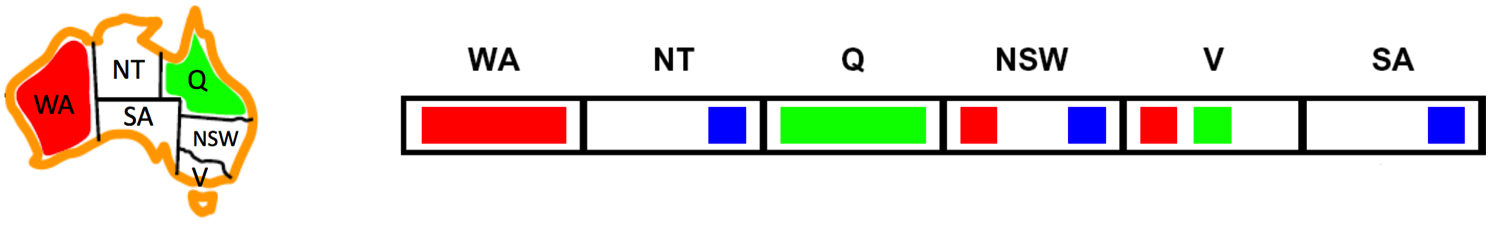
\includegraphics[width=16cm]{img/arc-consistency-ex-2.png}
		\end{center}
		Because we pruned a value from the domain of $V$, we need to enqueue all arcs with $V$ at the head - $SA \rightarrow V$, $NSW \rightarrow V$. Since $NSW \rightarrow V$ is already in $Q$, we only need to add $SA \rightarrow V$, leaving us with our updated queue
		\begin{eqnarray*}
		Q = [SA \rightarrow NSW, NSW \rightarrow SA, SA \rightarrow NT, NT \rightarrow SA, V \rightarrow NSW, NSW \rightarrow V, SA \rightarrow V]
		\end{eqnarray*}
		We can continue this process until we eventually remove the arc $SA \rightarrow NT$ from $Q$. Enforcing arc consistency on this arc removes $blue$ from $SA$'s domain, leaving it empty and triggering a backtrack.

	Arc consistency is typically implemented with the AC-3 algorithm (Arc Consistency Algorithm \#3), for which the pseudocode is as follows:
		\begin{center}
			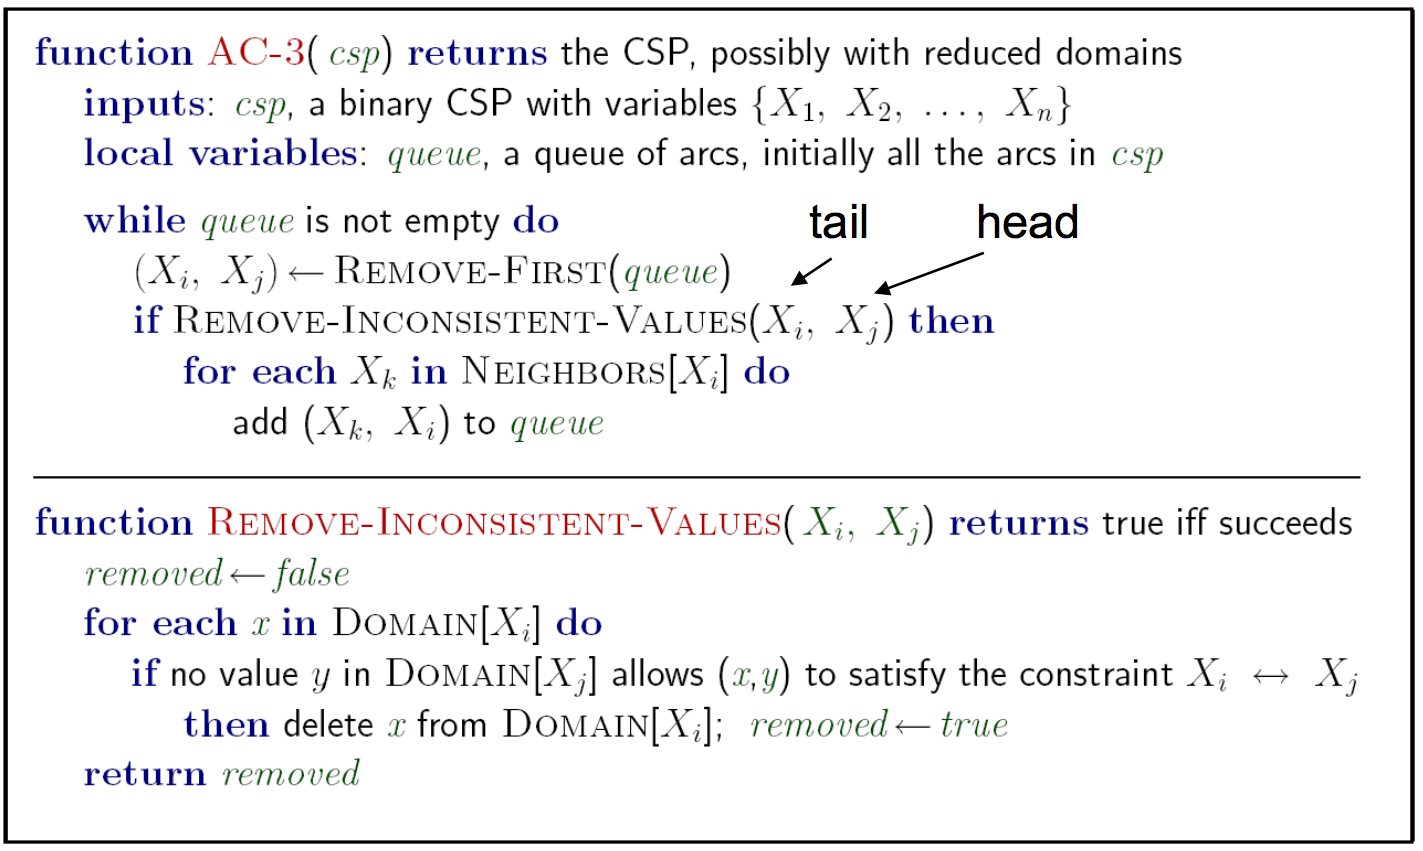
\includegraphics[width=12cm]{img/arc-consistency-pseudo.png}
		\end{center}
	Overall, arc consistency is more holistic of a domain pruning technique than forward checking and leads to fewer backtracks, but requires running significantly more computation in order to enforce. Accordingly, it's important to take into account this tradeoff when deciding which filtering technique to implement for the CSP you're attempting to solve.

	As an interesting parting note about consistency, arc consistency is a subset of a more generalized notion of consistency known as \textbf{k-consistency}, which when enforced guarantees that for any set of $k$ nodes in the CSP, a consistent assignment to any subset of $k-1$ nodes guarantees that the $k^{th}$ node will have at least one consistent value. This idea can be further extended through the idea of \textbf{strong k-consistency}. A graph that is strong $k$-consistent possesses the property that any subset of $k$ nodes is not only $k$-consistent but also $k-1, k-2, \hdots, 1$ consistent as well. Not surprisingly, imposing a higher degree of consistency on a CSP is more expensive to compute. Under this generalized definition for consistency, we can see that arc consistency is equivalent to $2$-consistency.

\subsection*{Ordering}
	We've delineated that when solving a CSP, we fix some ordering for both the variables and values involved. In practice, it's often much more effective to compute the next variable and corresponding value "on the fly" with two broad principles, \textbf{minimum remaining values} and \textbf{least constraining value}:
		\begin{itemize}
			\item \textit{Minimum Remaining Values (MRV)} - When selecting which variable to assign next, using an MRV policy chooses whichever unassigned variable has the fewest valid remaining values (the \textit{most constrained variable}). This is intuitive in the sense that the most constrained variable is most likely to run out of possible values and result in backtracking if left unassigned, and so it's best to assign a value to it sooner than later.
			\item \textit{Least Constraining Value (LCV)} - Similarly, when selecting which value to assign next, a good policy to implement is to select the value that prunes the fewest values from the domains of the remaining unassigned values. Notably, this requires additional computation (e.g. rerunning arc consistency/forward checking or other filtering methods for each value to find the LCV), but can still yield speed gains depending on usage.
		\end{itemize}

\subsection*{Structure}
	A final class of improvements to solving constraint satisfaction problems are those that exploit their structure. In particular, if we're trying to solve a \textbf{tree-structured CSP} (one that has no loops in its constraint graph), we can reduce the runtime for finding a solution from $O(d^N)$ all the way to $O(nd^2)$, linear in the number of variables. This can be done with the tree-structured CSP algorithm, outlined below:
		\begin{itemize}
			\item First, pick an arbitrary node in the constraint graph for the CSP to serve as the root of the tree (it doesn't matter which one because basic graph theory tells us any node of a tree can serve as a root).
			\item Convert all undirected edges in the tree to directed edges that point \textit{away} from the root. Then \textbf{linearize} (or \textbf{topologically sort}) the resulting directed acyclic graph. In simple terms, this just means order the nodes of the graph such that all edges point rightwards. Noting that we select node $A$ to be our root and direct all edges to point away from $A$, this process results in the following conversion for the CSP presented below:
		\end{itemize}
				\begin{center}
					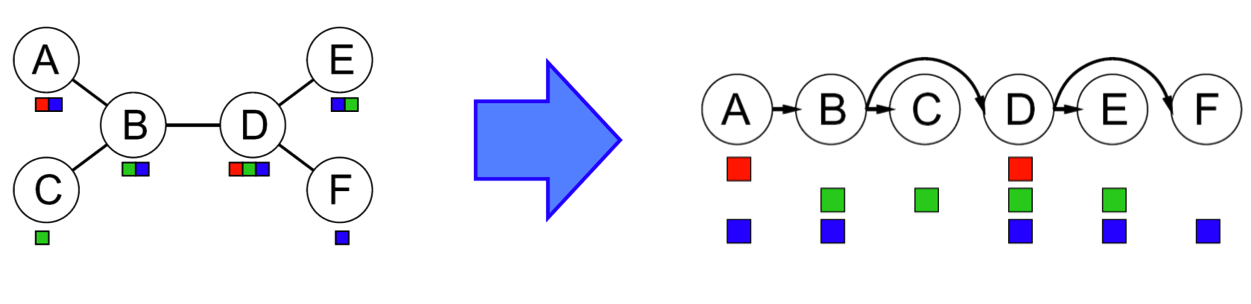
\includegraphics[width=15cm]{img/tree-structured-alg.png}
				\end{center} 
		\begin{itemize}
			\item Perform a \textbf{backwards pass} of arc consistency. Iterating from $i = n$ down to $i = 2$, enforce arc consistency for all arcs $Parent(X_i) \longrightarrow X_i$. For the linearized CSP from above, this domain pruning will eliminate a few values, leaving us with the following:
			\hspace{-8mm}
				\begin{center}
					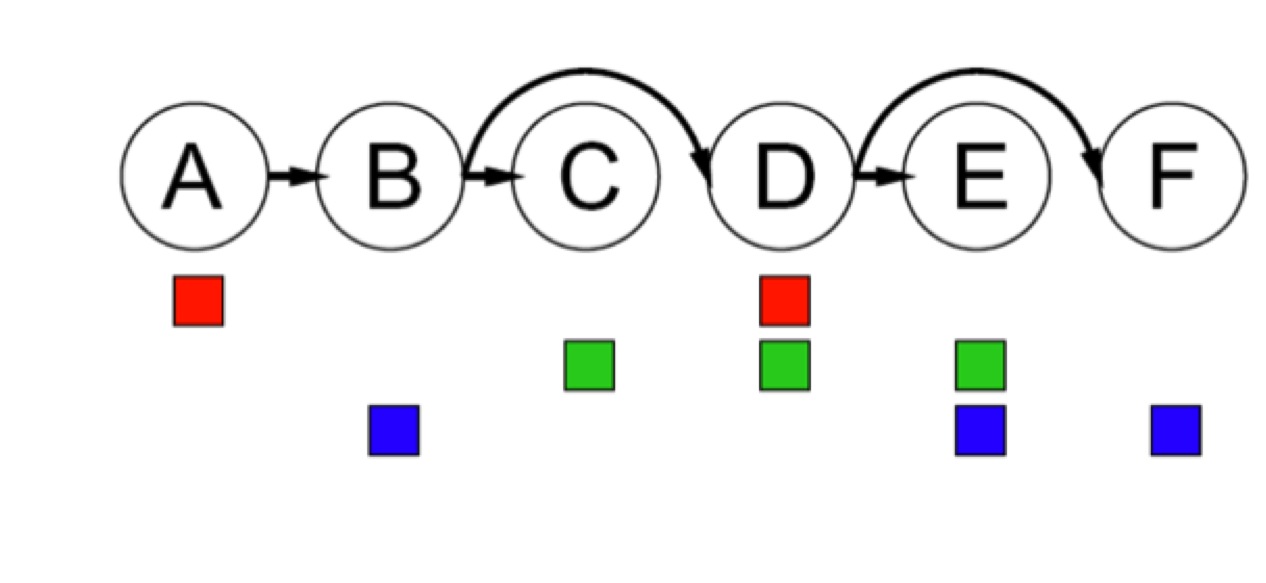
\includegraphics[width=8cm]{img/pruned-tree.png}
				\end{center}
			\vspace{-8mm}
			\item Finally, perform a \textbf{forward assignment}. Starting from $X_1$ and going to $X_n$, assign each $X_i$ a value consistent with that of its parent. Because we've enforced arc consistency on all of these arcs, no matter what value we select for any node, we know that its children will each all have at least one consistent value. Hence, this iterative assignment guarantees a correct solution, a fact which can be proven inductively without difficulty.
		\end{itemize}
	The tree structured algorithm can be extended to CSPs that are reasonably close to being tree-structured with \textbf{cutset conditioning}. Cutset conditioning involves first finding the smallest subset of variables in a constraint graph such that their removal results in a tree (such a subset is known as a \textbf{cutset} for the graph). For example, in our map coloring example, South Australia ($SA$) is the smallest possible cutset:
		\begin{center}
			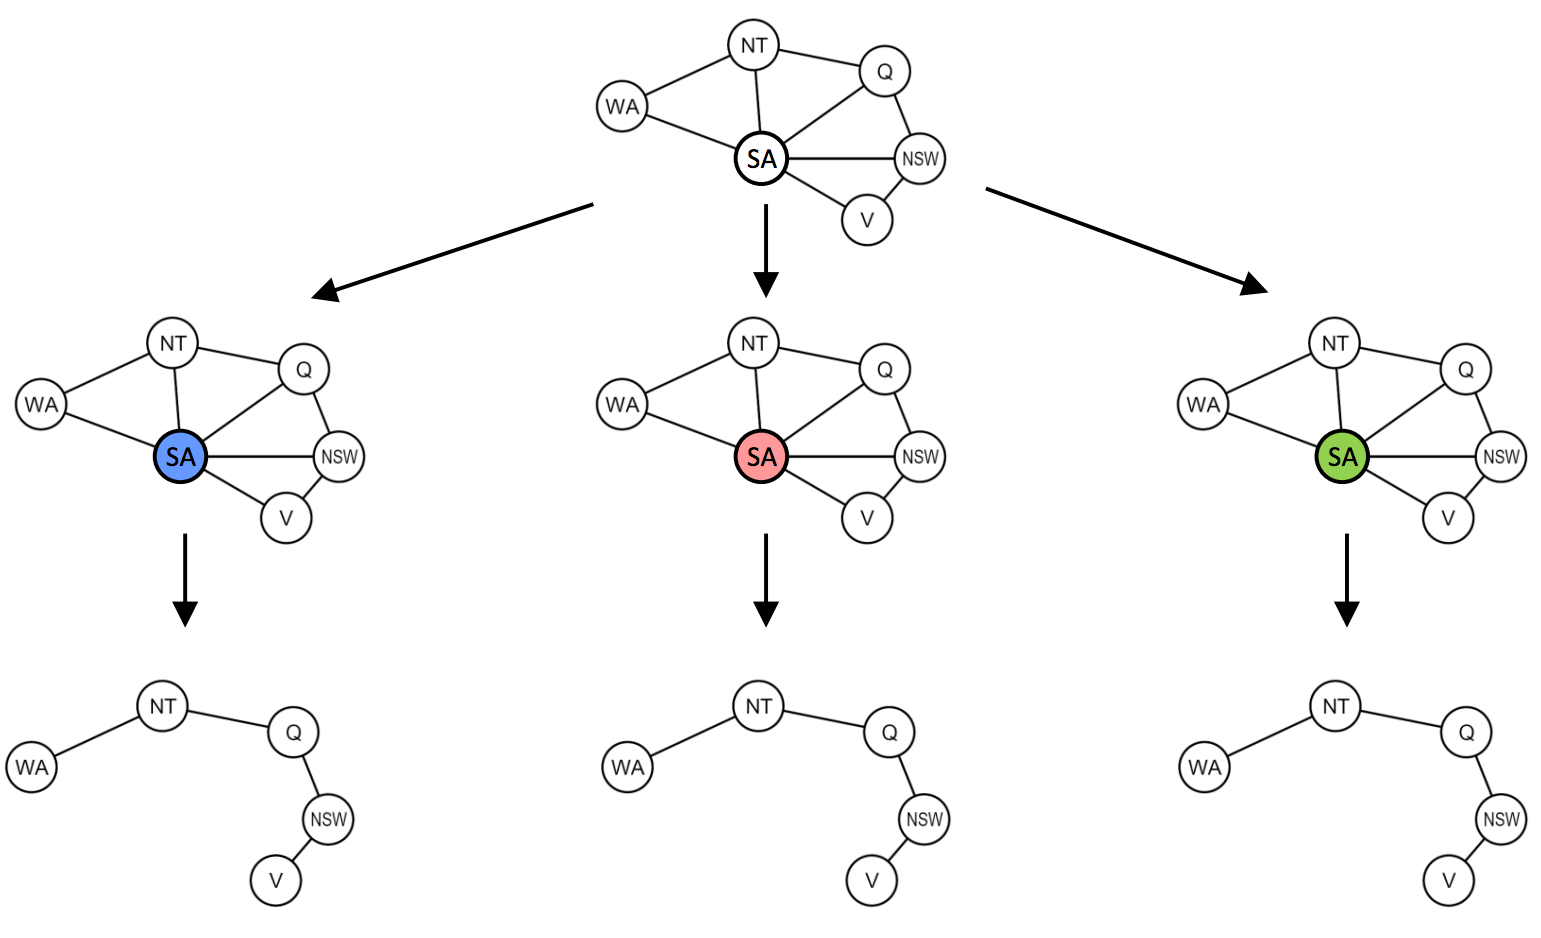
\includegraphics[width=14cm]{img/cutset.png}
		\end{center}
	Once the smallest cutset is found, we assign all variables in it and prune the domains of all neighboring nodes. What's left is a tree-structured CSP, upon which we can solve with the tree-structured CSP algorithm from above! The initial assignment to a cutset of size $c$ may leave the resulting tree-structured CSP(s) with no valid solution after pruning, so we may still need to backrack up to $d^c$ times. Since removal of the cutset leaves us with a tree-structured CSP with $(n - c)$ variables, we know this can be solved (or determined that no solution exists) in $O((n - c)d^2)$. Hence, the runtime of cutset conditioning on a general CSP is $O(d^c(n-c)d^2)$, very good for small $c$.

\subsection*{Iterative Improvement}
	As a final topic of interest, backtracking search is not the only algorithm that exists for solving constraint satisfaction problems. Another widely used class of algorithms is \textbf{iterative improvement}, for which the idea is childishly simple but remarkably useful. Iterative improvement works by starting with some random assignment to values then selecting the variable that violates the most constraints and resetting it to the value that violates the fewest constraints (a policy known as the \textbf{min-conflicts heuristic}). Under such a policy, constraint satisfaction problems like $N$-queens becomes very fast and efficient to solve. For example, in following example with $4$ queens, we arrive at a solution after only 2 iterations:
		\begin{center}
			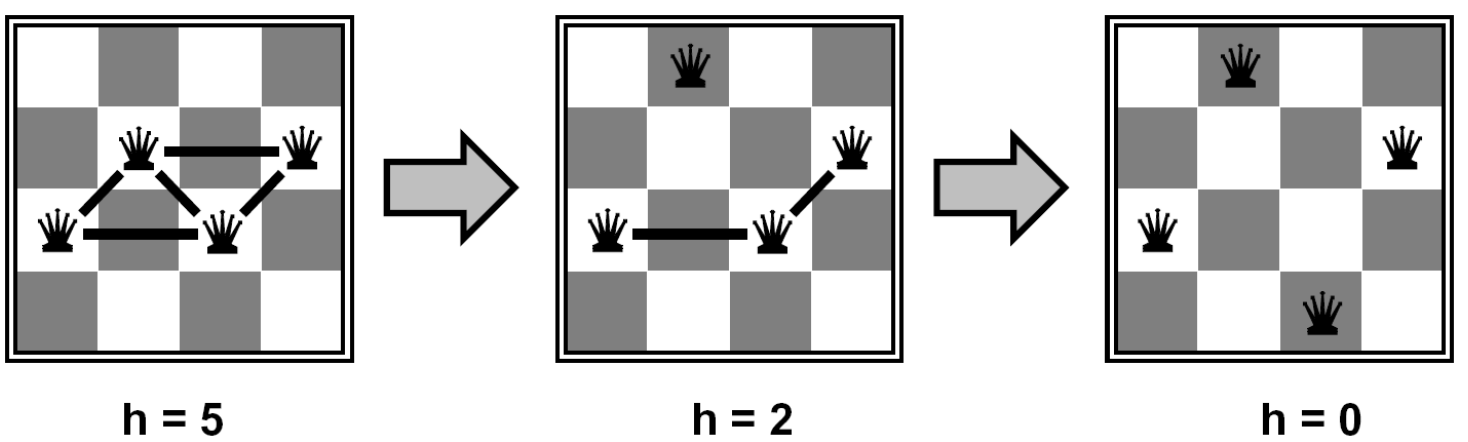
\includegraphics[width=10cm]{img/four-queens.png}
		\end{center}
	In fact, iterative improvement appears to run in almost constant time and have a high probability of success not only for $N$-queens with arbitrarily large $N$, but also for any randomly generated CSP! The primary caveat is that using iterative improvement is extremely expensive in a narrow range for the following ratio:
		\begin{center}
			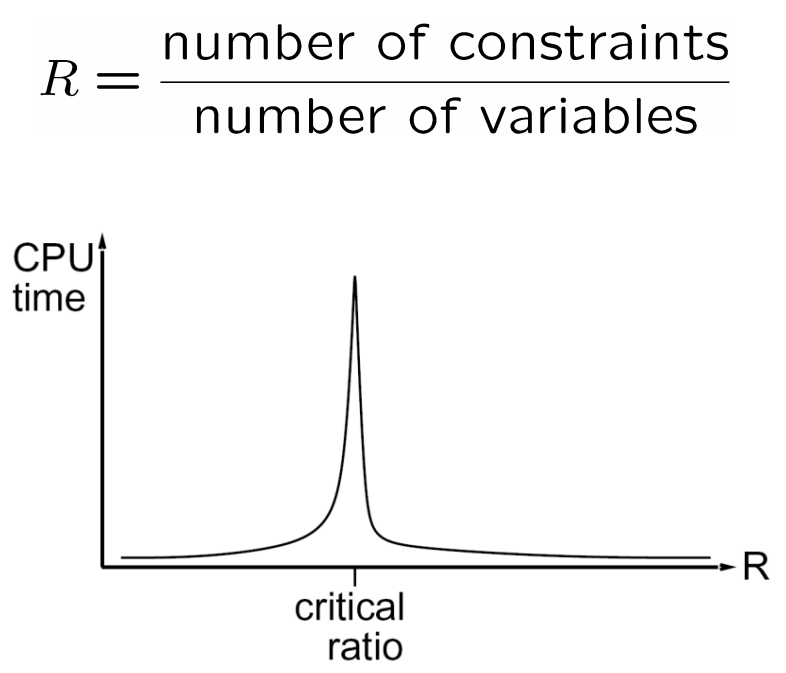
\includegraphics[width=7cm]{img/critical-ratio.png}
		\end{center}

\newpage
\section*{Summary}
	It's important to remember that constraint satisfaction problems in general do not have an efficient algorithm which solves them in polynomial time with respect to the number of variables involved. However, by using various heuristics, we can often find solutions in an acceptable amount of time:
		\begin{itemize}
			\item \textit{Filtering} - Filtering handles pruning the domains of unassigned variables ahead of time to prevent unnecessary backtracking. The two important filtering techniques we've covered are \textit{forward checking} and \textit{arc consistency}.
			\item \textit{Ordering} - Ordering handles selection of which variable or value to assign next to make backtracking as unlikely as possible. For variable selection, we learned about a \textit{MRV policy} and for value selection we learned about a \textit{LCV policy}.
			\item \textit{Structure} - If a CSP is tree-structured or close to tree-structured, we can run the tree-structured CSP algorithm on it to derive a solution in linear time. Similarly, if a CSP is close to tree structured, we can use \textit{cutset conditioning} to transform the CSP into one or more independent tree-structured CSPs and solve each of these separately.
		\end{itemize}

\end{document}